% Created 2016-08-17 Wed 14:38
\documentclass[tikz]{standalone}

\usepackage[utf8]{inputenc}
\usepackage[T1]{fontenc}

\usepackage{circledsteps}

\RequirePackage{xcolor}

%% HPI color definitions according to the design manual
% These do not exactly match the RGB values used in the Powerpoint slide master due to unknown reasons
\definecolor{hpiyellow}{RGB}{246,168,0}
\definecolor{hpiorange}{RGB}{221,97,8}
\definecolor{hpired}{RGB}{177,6,58}
\definecolor{hpigray}{RGB}{90,96,101}
\definecolor{hpiblue}{RGB}{0,122,158}


\renewcommand{\sfdefault}{neosans}
% Different font weights for neosans
\newcommand{\textl}[1]{{\fontseries{l}\selectfont #1}} % light
\newcommand{\textm}[1]{{\fontseries{m}\selectfont #1}} % medium, same as default weight
\newcommand{\textsb}[1]{{\fontseries{sb}\selectfont #1}} % semibold
\newcommand{\textmb}[1]{{\fontseries{mb}\selectfont #1}} % bold, same as \textbf
\newcommand{\texteb}[1]{{\fontseries{eb}\selectfont #1}} % extra bold
\newcommand{\textub}[1]{{\fontseries{ub}\selectfont #1}} % ultra bold

\tikzset{every picture/.style={/utils/exec={\sffamily}}}
\tikzset{flipflop RSflanke/.style={
  flipflop,
  flipflop def={t1=S, t2=C, c2=1, t3=R, t6=Q, t4={\ctikztextnot{Q}}}
}}


\tikzset{
  mechanicalSwitch/.pic={
    \coordinate (-inUp) at (135:2); 
    \coordinate (-inDown) at (235:2);
    \coordinate (-out) at (2,0);
    \coordinate (-center) at (0,0);
    
    \draw (0,0) circle [radius = 2cm];
    \draw [fill=gray!20] (0,0) circle [radius = 0.2cm];

    \draw (0, 0) -- (2, 0);
    \draw (135:.8) -- (135:2); 
    \draw (225:.8) -- (225:2); 

    \draw [fill=gray!20] (2, 0) circle [radius=0.05cm]; 
    \draw [fill=gray!20] (135:2) circle [radius=0.05cm]; 
    \draw [fill=gray!20] (225:2) circle [radius=0.05cm]; 

    
    \draw [thick] (0,0) -- (175:1.5); 

    \draw [dashed, <->, domain=135:225] plot ({cos(\x)}, {sin(\x)}); 
  },
  mechanicalSwitchClosed/.pic={
    \coordinate (-inUp) at (135:2); 
    \coordinate (-inDown) at (255:2);
    \coordinate (-out) at (2,0);
    \coordinate (-center) at (0,0);
    \draw (0,0) circle [radius = 2cm];
    \draw [fill=gray!20] (0,0) circle [radius = 0.2cm];

    \draw (0, 0) -- (2, 0);
    \draw (135:.8) -- (135:2); 
    \draw (225:.8) -- (225:2); 

    \draw [fill=gray!20] (2, 0) circle [radius=0.05cm]; 
    \draw [fill=gray!20] (135:2) circle [radius=0.05cm]; 
    \draw [fill=gray!20] (225:2) circle [radius=0.05cm]; 

    
    \draw [thick] (0,0) -- (135:2); 

    \draw [dashed, <->, domain=135:225] plot ({cos(\x)}, {sin(\x)}); 
  }
}


\usetikzlibrary{calc}
\usetikzlibrary{positioning}


\usetikzlibrary{calc}

\usepackage{pgfplots}
% \usepackage{pgfplotstable}

\usetikzlibrary{pgfplots.patchplots}

\begin{document}

\pgfplotsset{every axis/.append style={
    font=\large,
    line width=1pt,
    tick style={line width=0.8pt}}}


 
% \pgfplotstableread{randomcurve.dat}\randomcurve

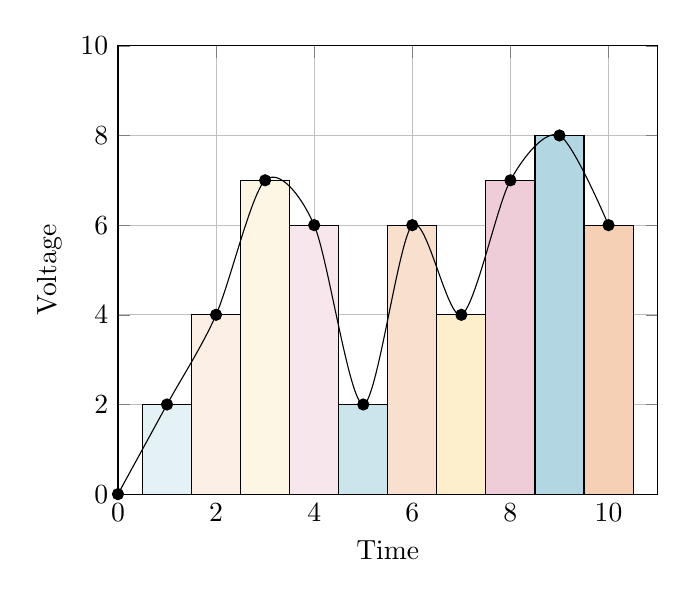
\begin{tikzpicture}
  \label{page:phy:averages:time}
\begin{axis}
    [grid=major,
    xlabel=Time,
    ylabel=Voltage,
    ymin = 0,
    ymax = 10,
    xmin = 0,     
    % xtick= {0, 1, 2, 3, 4,5},
    ]

  \draw [thin, fill=hpiblue!10] (axis cs: 0.5, 0) rectangle (axis cs: 1.5, 2); 
  \draw [thin, fill=hpiorange!10] (axis cs: 1.5, 0) rectangle (axis cs: 2.5, 4); 
  \draw [thin, fill=hpiyellow!10] (axis cs: 2.5, 0) rectangle (axis cs: 3.5, 7); 
  \draw [thin, fill=hpired!10] (axis cs: 3.5, 0) rectangle (axis cs: 4.5, 6); 
  \draw [thin, fill=hpiblue!20] (axis cs: 4.5, 0) rectangle (axis cs: 5.5, 2); 
  \draw [thin, fill=hpiorange!20] (axis cs: 5.5, 0) rectangle (axis cs: 6.5, 6); 
  \draw [thin, fill=hpiyellow!20] (axis cs: 6.5, 0) rectangle (axis cs: 7.5, 4); 
  \draw [thin, fill=hpired!20] (axis cs: 7.5, 0) rectangle (axis cs: 8.5, 7); 
  \draw [thin, fill=hpiblue!30] (axis cs: 8.5, 0) rectangle (axis cs: 9.5, 8); 
  \draw [thin, fill=hpiorange!30] (axis cs: 9.5, 0) rectangle (axis cs: 10.5, 6); 

  \addplot [smooth, mark=*] table {
    0 0 
      1 2
      2 4
      3 7
      4 6
      5 2
      6 6
      7 4
      8 7
      9 8
      10 6
    };

  \end{axis}
\end{tikzpicture}

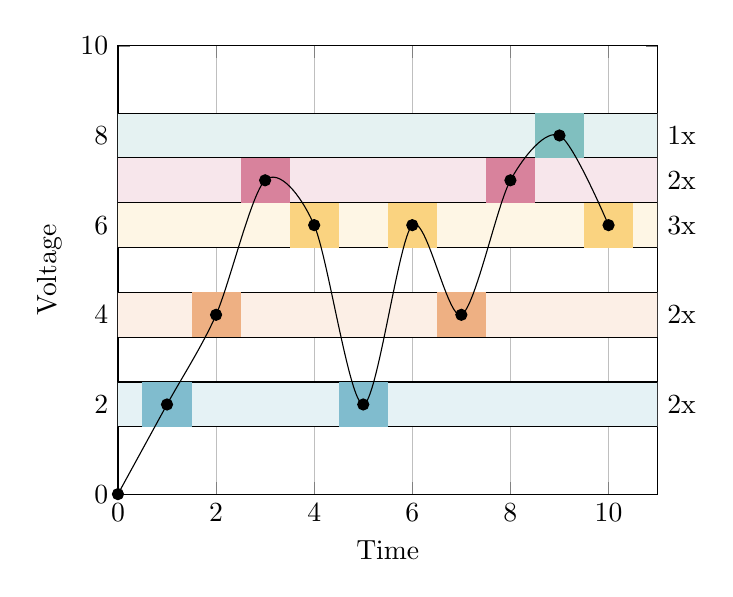
\begin{tikzpicture}
  \label{page:phy:averages:values}
  
  \begin{axis}
    [grid=major,
    xlabel=Time,
    ylabel=Voltage,
    ymin = 0,
    ymax = 10,
    xmin = 0, 
    % xtick= {0, 1, 2, 3, 4,5},
    ]

  \draw [thin, fill=hpiblue!10] (axis cs: -1, 1.5) rectangle (axis cs: 11, 2.5); 
  \draw [draw=none, fill=hpiblue!50] (axis cs: 0.5, 1.5) rectangle (axis cs: 1.5, 2.5); 
  \draw [draw=none, fill=hpiblue!50] (axis cs: 4.5, 1.5) rectangle (axis cs: 5.5, 2.5); 
  \node at (axis cs: 11, 2)  (zwei) {}; 

  \draw [thin, fill=hpiorange!10] (axis cs: -1, 3.5) rectangle (axis cs: 11, 4.5); 
  \draw [draw=none, fill=hpiorange!50] (axis cs: 1.5, 3.5) rectangle (axis cs: 2.5, 4.5); 
  \draw [draw=none, fill=hpiorange!50] (axis cs: 6.5, 3.5) rectangle (axis cs: 7.5, 4.5); 

  \node at (axis cs: 11, 4)  (vier) {}; 


  \draw [thin, fill=hpiyellow!10] (axis cs: -1, 5.5) rectangle (axis cs: 11, 6.5); 
  \draw [draw=none, fill=hpiyellow!50] (axis cs: 3.5, 5.5) rectangle (axis cs: 4.5, 6.5); 
  \draw [draw=none, fill=hpiyellow!50] (axis cs: 5.5, 5.5) rectangle (axis cs: 6.5, 6.5); 
  \draw [draw=none, fill=hpiyellow!50] (axis cs: 9.5, 5.5) rectangle (axis cs: 10.5, 6.5); 

  \node at (axis cs: 11, 6)  (sechs) {}; 

  \draw [thin, fill=hpired!10] (axis cs: -1, 6.5) rectangle (axis cs: 11, 7.5); 
  \draw [draw=none, fill=hpired!50] (axis cs: 2.5, 6.5) rectangle (axis cs: 3.5, 7.5); 
  \draw [draw=none, fill=hpired!50] (axis cs: 7.5, 6.5) rectangle (axis cs: 8.5, 7.5); 

  \node at (axis cs: 11, 7)  (sieben) {}; 

  \draw [thin, fill=teal!10] (axis cs: -1, 7.5) rectangle (axis cs: 11, 8.5); 
  \draw [draw=none, fill=teal!50] (axis cs: 8.5, 7.5) rectangle (axis cs: 9.5, 8.5); 


  \node at (axis cs: 11, 8)  (acht) {}; 
  

  \addplot [smooth, mark=*] table {
    0 0 
      1 2
      2 4
      3 7
      4 6
      5 2
      6 6
      7 4
      8 7
      9 8
      10 6
    };

  \end{axis}

  \node [anchor=west] at (zwei) {2x}; 
  \node [anchor=west] at (vier) {2x}; 
  \node [anchor=west] at (sechs) {3x}; 
  \node [anchor=west] at (sieben) {2x}; 
  \node [anchor=west] at (acht) {1x}; 

  
\end{tikzpicture}



\end{document}